\documentclass[a4paper,twoside,12pt,nochapterprefix]{scrbook}

\usepackage{amsmath,amssymb,amsthm}
\usepackage[footnotesize,sl,SL,hang,tight]{subfigure}  % helpful package for aligning figures next to each other
\usepackage{longtable} % tables over several pages
\usepackage[font={small,sl},hang,labelfont=bf]{caption} % configure captions
\usepackage{booktabs} % publication quality tables for LaTeX
\newcommand{\ra}[1]{\renewcommand{\arraystretch}{#1}}

\Ifpdfoutput{%
	\usepackage[pdftex]{graphicx}
	\usepackage[]{pdfpages} %for including full pdf pages
}{%
	\usepackage{graphicx}
}
\usepackage{rotating} % rotate figures

\usepackage{scrlayer-scrpage}

% Meta Post
\usepackage{emp}
\DeclareGraphicsRule{.1}{mps}{*}{} 
\DeclareGraphicsRule{.2}{mps}{*}{} 

% Listings
\usepackage{listings}
\lstset{
    language=C++,
    basicstyle=\ttfamily,
    keywordstyle=\color{blue}\ttfamily,
    stringstyle=\color{red}\ttfamily,
}

% tikz
\usepackage{lscape}
\usepackage{tikz}
\usepackage[underline=true,rounded corners=false]{pgf-umlsd}

% Font packages:
\usepackage{times}
\usepackage{helvet}   % sets sans serif font
\usepackage[T1]{fontenc}
\newcommand{\Cpp}{C\nolinebreak[4]\hspace{-.05em}\raisebox{.15ex}{\bf ++}\hspace{.2em}} % C++ macro

%PDF hyperref config
\Ifpdfoutput{%
	\usepackage[pdftex,
		a4paper,
		bookmarks,
		bookmarksopen=true,
		bookmarksnumbered=true,
		pdfauthor={Sven Kellenberger},       % FILL THIS IN PROPERLY
		pdftitle={Thesis Title},   % FILL THIS IN PRPERLY
		colorlinks,
		linkcolor=black,
		citecolor=black,
		filecolor=black,
		urlcolor=black,
		anchorcolor=black,
		menucolor=black,
		breaklinks=true,
		pageanchor=true,
		plainpages=false,
		pdfpagelabels=true]{hyperref}
}{}

\Ifpdfoutput{%
	\pdfcompresslevel=9
	\pdfoutput=1
	\DeclareGraphicsExtensions{.pdf,.png}
}{}

\bibliographystyle{acmsiggraph}


% A4
%
\topmargin -0.5in
\textheight 9.3in
\textwidth 6.3in
\oddsidemargin 0.18in
\evensidemargin -0.22in
\parskip 0.1in
\parindent 0in

\renewcommand{\arraystretch}{1.5}
\renewcommand{\baselinestretch}{1}

% TO DO search symbol
\newcommand{\TODO}{\mbox{\large\bf TO DO}}
\newcommand{\REFR}{\mbox{\large\bf REFR}}

%  Terminates current page and paragraph, makes sure next page starts on
%  an odd-number, and generates a completely blank page, without page markers,
%  if necessary.
\newcommand{\clearemptydoublepage}{\newpage{\pagestyle{empty}\cleardoublepage}}


% Stripped from acm siggraph bst and cls
\makeatletter

% no labels in bibliography.
\def\@biblabel#1{}

\newlength{\bibhang}
\setlength{\bibhang}{1em}

% Change in-bibliography biberence style
\def\thebibliography#1{%
  \section*{%
    \bibname\@mkboth{\sl\uppercase{\bibname}}{\sl\uppercase{\bibname}}}
  \list{\relax}{\setlength{\labelsep}{0em}
                \setlength{\itemindent}{-\bibhang}
                \setlength{\leftmargin}{\bibhang}}
  \def\newblock{\hskip .11em plus .33em minus .07em}
  \sloppy\clubpenalty4000\widowpenalty4000
  \sfcode`\.=1000\relax}

% Not sure what this does...
%\def\@citex[#1]#2{\if@filesw\immediate\write\@auxout{\string\citation{#2}}\fi
%  \def\@citea{}\@cite{\@for\@citeb:=#2\do
%    {\@citea\def\@citea{; }\@ifundefined
%      {b@\@citeb}{{\bf ?}\@warning
%      {Citation '\@citeb' on page \thepage \space undefined}}%
%{\csname b@\@citeb\endcsname}}}{#1}}

% Change in-document citation styles
\let\@internalcite\cite
\def\cite{\def\citename##1{##1}\@internalcite}
\def\shortcite{\def\citename##1{}\@internalcite}

\makeatother


\begin{document}

%% Define leading chapter pages
%
\addtokomafont{chapter}{\setlength{\parskip}{190pt}}   % SEVERE HACK to keep spacing to chapter art work
%\addtokomafont{chapter}{\rmfamily}        % remove this if you prefer sans-serif section titles
%\addtokomafont{section}{\rmfamily}        % remove this if you prefer sans-serif section titles
%\addtokomafont{subsection}{\rmfamily}     % remove this if you prefer sans-serif section titles
%\addtokomafont{subsubsection}{\rmfamily}  % remove this if you prefer sans-serif section titles
%\addtokomafont{paragraph}{\rmfamily}      % replace by \sffamily if you prefer sans-serif para titles
\addtokomafont{paragraph}{\sffamily}

\def\mychpstyleintl{%
{\noindent\setlength{\tabcolsep}{0pt}\setlength{\arrayrulewidth}{2pt}%
\begin{tabular}{c}
\\[100pt]
\begin{tabular}{lr}
\begin{tabular}{p{0.6\linewidth}}
\\
\end{tabular}
&
\begin{tabular}{p{0.4\linewidth}}
\rightline{{%
\sffamily%
\fontseries{bx}%
\fontshape{n}%
\fontsize{100}{120}%choose baselineskip to be 1.2 times font size
\selectfont
\thechapter}}
\end{tabular}
\end{tabular}\\[-250pt]
\end{tabular}
}}

\newpagestyle{mychapterpagestyle}{{\protect\mychpstyleintl}{\protect\mychpstyleintl}}{}
\newpagestyle{myappendixpagestyle}{{\protect\mychpstyleintl}{\protect\mychpstyleintl}}{}
%%

%% macros e.g.
\newcommand{\mfytext}[0]{my fancy text}

%refs
\newcommand{\chpref}[1]{Chapter \ref{#1}}
\newcommand{\secref}[1]{Section \ref{#1}}
%\newcommand{\equref}[1]{Equation \ref{#1}} %better use builtin \eqref{}
\newcommand{\figref}[1]{Figure \ref{#1}}
\newcommand{\tabref}[1]{Table \ref{#1}}
\newcommand{\apxref}[1]{Appendix \ref{#1}}
%%

%% Replace this by your own design of a title page
%
%\title{Thesis Title}
%\author{My Name}
%\date{September 2042}
%\maketitle
%\clearemptydoublepage
% --- selfmade version ----
\begin{titlepage}
	\topmargin 1.0cm
	\oddsidemargin 0.0cm
	\evensidemargin 0.0cm
	%\textwidth 6.5in
	\centering
	\Huge
	\vspace{3.0cm}
	\textbf{\textsf{Object Tracking on the HoloLens}} \\[2.0cm]
	\includegraphics*[width=0.8\textwidth]{figures/teaser.jpg} \\ % TITLE IMAGE - replace by attractive and representative images from your thesis
	\vspace{3cm}
	\sffamily
	\Large
	Sven Kellenberger
	\\[0.8cm]
	\large
	Master Thesis % Bachelor Thesis
	\\
	April 2021
	\\[1.3cm]
	\emph{Supervisors:}\\
	Dr.\ Roi Poranne\\
	Dr.\ Timothy Sandy \\% The name of the thesis supervisor
	Prof.\ Dr.\ Stelian Coros		% The supervising professor
	\vfill
	\includegraphics*[width=0.3\textwidth]{figures/ETH_logo} \hfill
	\includegraphics*[width=0.3\textwidth]{figures/CRL_logo}
	\vspace{3.4cm}
\end{titlepage}
\clearemptydoublepage
%%

\pagenumbering{roman}
\setcounter{page}{1}

\chapter*{Abstract}

Using computer vision algorithms to track objects in variable three-dimensional environments and using the found poses to guide complex construction tasks is an interesting area of research which opens up a lot of exciting possibilities. If the construction is performed by a human using a mixed reality headset promises great flexibility an easy of use.

In this thesis I integrate a preexisting object tracking library into the HoloLens 2 ecosystem and build a small application with a simple user interface. This application enables the user to use object tracking to accurately build a simple brick tower by hand. To accomplish this, I make use of various Windows APIs and the new Research Mode for HoloLens 2 to provide the Object Tracker with the data streams it needs.

\cleardoublepage
\chapter*{Zusammenfassung}

Das Tracking von Objekten in variablen drei-dimensionalen Umgebungen zur Unterstützung von Bauvorhaben von komplexen Konstruktionen ist ein aktives Forschungsgebiet, welches viele spannende Möglichkeiten bietet. Für Fälle, wo die Konstruktion von einem Menschen per Hand ausgeführt wird, ist es für die höchstmögliche Flexibilität vielversprechend, ein  Mixed-Reality Headset einzusetzen.

In dieser Arbeit integriere ich eine bereits existierende Objekt-Tracking Library in das Ökosystem der HoloLens 2 und baue eine kleine Applikation mit einem einfachen User Interface. Diese Applikation kann genutzt werden, um einen kleinen Turm aus Bauklötzen mit grosser Präzision per Hand zu konstruieren. Um dieses Zeil zu erreichen verwende ich verschiedene Windows APIs und den neuen Research Mode für die HoloLens 2, um den Objekt-Tracker mit den nötigen Datenströmen zu versorgen.


%-----------------------------------------------------------------------------------------------
%include task description here:
\cleardoublepage
%-----------------------------------------------------------------------------------------------

%include acknowledgment here:
%\include{acknowledgment}

\tableofcontents

\cleardoublepage
\phantomsection
\addcontentsline{toc}{chapter}{List of Figures}
\listoffigures

\cleardoublepage
\phantomsection
\addcontentsline{toc}{chapter}{List of Tables}
\listoftables
\cleardoublepage

\pagenumbering{arabic}
\renewcommand*{\chapterpagestyle}{mychapterpagestyle}
\renewcommand*{\chapterformat}{} % show chapter titles only (no numbers)
% \setchapterpreamble[o]{...}  unfortunately does not move the \chapter output downwards

% ---- MAIN PART ----

% set counter to n-1:
\setcounter{chapter}{0}

\chapter{Introduction}

In our world today we rely more and more on algorithms to help us achieve our goals. We use auto-correction to avoid typos in our text messages, we let Netflix suggest the best matching movies dependent on our tastes to us and we rely on robots to run fully automated assembly lines to produce everyday products. However, all these examples have in common that they run in well defined ecosystems where most external parameters can be controlled and the remaining ones can be accounted for. As soon as we try to tackle problems where it is not possible to control most external factors, we need more robust algorithms which are naturally harder to develop.

One such problem is the construction of complex structures in unknown environments such as building sites. In \cite{ViObjectTracker} the authors propose a framework which enables real-time tracking of a sensor-head relative to multiple objects and use it to help constructing complex brick structures by hand. In this thesis, I will build on this work and incorporate the existing code into a mixed reality application which can be run on a mixed reality headset. This allows for easy use without the need of holding a camera and other sensors.

\section{Mixed Reality}

The field of computer vision concerns itself with algorithms analysing images and videos to extract as much information as possible about the depicted three-dimensional environment. Within computer vision, mixed reality is a very active area of research. While virtual reality creates a virtual three-dimensional space in which the user can move around and interact with objects, mixed reality incorporates virtual elements into the real world and lets virtual and real objects interact with each other and the user. Its applications range from video games to semi-virtual meetings to supporting surgeons by visualizing CT scans.

Specifically developed headsets are used to provide the most immersive mixed reality experience. One such headset is the HoloLens which was first launched in 2016 by Microsoft and its successor the HoloLens 2, launched in 2019. Equipped with state of the art sensors to allow for spatial orientation as well as fully articulated hand tracking and eye gaze tracking, the HoloLens 2 is able to run complex programs, helping the user perform various tasks \cite{HololensHardware}. 

In this thesis I make use of the low level sensor streams of the HoloLens 2 available via Resarch Mode~\cite{ResearchMode} to provide the aforementioned code with the sensor data streams it requires. I also build a small application which visualizes the state of the Object Tracker and enables the user to interact with it.
% set counter to n-1:
\setcounter{chapter}{1}

\chapter{Related Work}

\section{HoloLens 2}

\begin{figure}
    \centering
    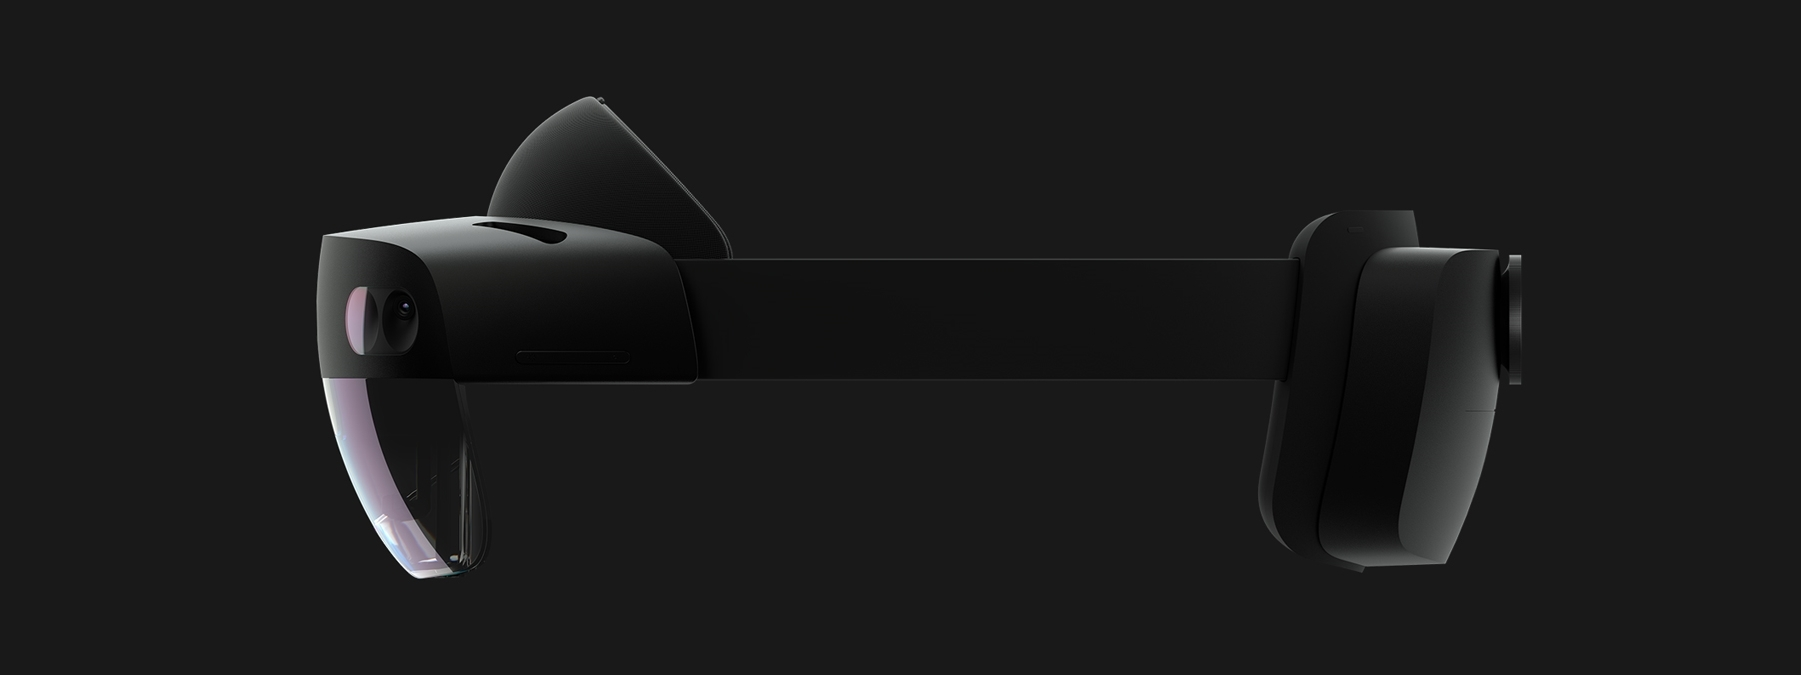
\includegraphics[width=0.9\linewidth]{figures/hololens.jpg}
    \caption[Side view of the HoloLens 2]{Side view of the HoloLens 2. Directly taken from \cite{HololensOverview}.}
      \label{fig:hololens}
\end{figure}

The HoloLens 2 (see fig. \ref{fig:hololens}) is a mixed reality headset developed by Microsoft and launched in 2019. It's the successor to the original HoloLens which was launched in 2016. Among the improvements are a larger field-of-view, fully articulated hand tracking, eye gaze tracking and a custom deep neural network core \cite{ResearchMode}. The HoloLens 2 runs Windows~10 and developers can create mixed reality apps by placing holograms in 3D space. See-through holographic lenses allow for an immersive mixed reality experience \cite{HololensHardware}.

\subsection{Hardware} \label{sec:holHardware}

The HoloLens 2 is designed to enable the creation of immersive mixed reality applications. It therefore is equipped with a lot of different sensors \cite{ResearchMode, HololensHardware}, some of them are:

\begin{itemize}
    \item RGB camera: Runs at up to 30fps with a resolution of up to 1080p. Able to take 8-MP photos.
    \item Depth camera: Is able to operate in two modes: Long Throw, which is a low-framerate ($\leq5$fps), far-depth mode and AHAT (Articulated HAnd Tracking) which is a high-framerate (45fps), near-depth mode.
    \item Four visible-light tracking (VLC) cameras: Placed at the left and right side of the headset and used for head tracking. Have a very wide field-of-view and produce greyscale images.
    \item Inertial Measurement Unit (IMU): Consists of an accelerometer, a gyroscope and a magnetometer. The accelerometer measures the linear acceleration, the gyroscope the rotation and the magnetometer the absolute orientation of the headset.
\end{itemize}

The placement of these sensors can be seen in fig. \ref{fig:holHardware}.

\begin{figure}
    \centering
    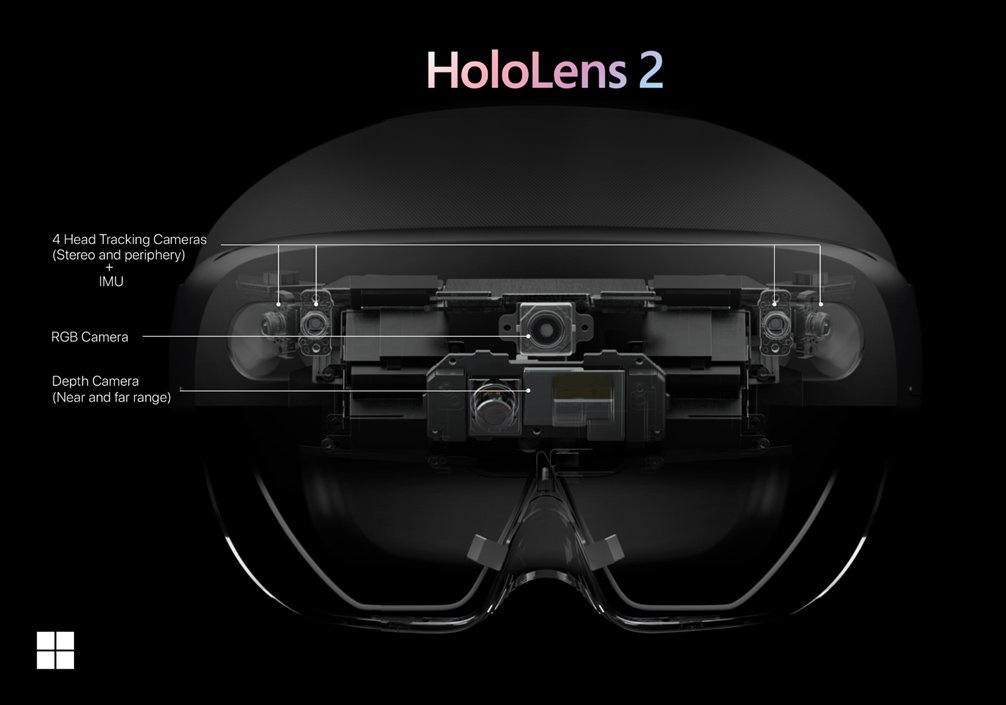
\includegraphics[width=0.9\linewidth]{figures/hololens2-front-view.png}
    \caption[Hololens 2 Hardware]{Image depicting the HoloLens 2 and some of its sensors, directly taken from Microsoft Docs \cite{HololensHardware}.}
      \label{fig:holHardware}
\end{figure}

The headset uses its various sensors to provide articulated hand tracking, eye gaze tracking, head tracking as well as spatial mapping out of the box. These tasks are performed by a special holographic processing unit with a deep neural network core which runs all native computer vision algorithms of the device. An additional Qualcomm Snapdragon 850 CPU is provided to run third-party applications. 

\subsection{Research Mode} \label{sec:ResearchMode}

The Windows Mixed Reality APIs \cite{DocMixedReality} provide access to a lot of functionality of the HoloLens 2 such as the capturing of camera frames and tracking of the the current head pose. However, these APIs don't allow for the developer to access the raw data streams of most sensors but only to the results of the processing of said streams for example the current head pose which is calculated using ineratial measurements. To address this, Microsoft introduced the Research Mode for HoloLens 2 \cite{ResearchMode} with the goal of encouraging contributions in the field of mixed reality by industrial and academic researchers. Research Mode needs to be specifically enabled in the Device Portal of the HoloLens 2 \cite{DevicePortal} and is not meant for applications targeted at end-users since they won't be able to run it. When enabled, Research Mode provides a set of \Cpp APIs to access various sensor streams of the HoloLens 2. Sensors exposed by Research Mode are the following:

\begin{itemize}
    \item VLC camera sensor: Provides access to the greyscale images produced by these cameras. Each camera can be targeted individually.
    \item Depth camera sensor: Provides access to the computed depth data for both modes described in sec. \ref{sec:holHardware} individually while also providing the raw infrared stream used to compute the depth map for both modes.
    \item IMU sensors: Provides access to measurement samples for each indiviual sensor. The API provides batches of measurement samples at a frequency between 12Hz and 22Hz.
\end{itemize}

Camera sensors and IMU sensors expose different functions. For example IMU sensors expose functions to either retrieve a single measurement sample per frame or a batch of measurement samples while camera sensors expose functions to map points from the three-dimensional camera space into the two-dimensional image space.

The API also provides extrinsic transformation matrices for each sensor relative to a static rigid node on the headset which represents the device origin and corresponds to the left front VLC camera. Each sensor returns a 4x4 transformation matrix to the this rigid node. To locate the sensors relative to other coordinate systems Research Mode allows for the retrieval of the GUID of the rigid node which can then be located relative to different coordinate systems using the HoloLens Perception API \cite{HololensPerception}. 

The authors of the Research Mode paper also provided a Github repository \cite{GithubRepoHololens2ForCV} which contains the full documentation for Research Mode as well as different example programs showcasing the use of Research Mode and code samples which can be used to develop with Research Mode.

\subsection{Development}

There are multiple options to develop mixed reality applications for HoloLens 2 \cite{DevMixedReality}. The most convenient ways are using one of the game engines Unity~\cite{Unity} or Unreal~\cite{Unreal}. Unity is especially well supported and runs the Mixed Reality Toolkit (MRTK) \cite{UnityMRTK} which is an open-source, cross-platform development kit for developing mixed reality applications. However there are multiple problems, when developing with Unity.

For one, Unity runs on C\# code while the used preexisting code for object tracking (see sec. \ref{sec:objectTracker}) is written in \Cpp. While it is possible to run DLLs (dynamic link libraries) compiled from \Cpp in Unity, the HoloLens 2 needs those DLLs to be compiled for UWP (Universal Windows Platform) and the ARM64 CPU architecture. Unity can run neither of those things in its built-in editor. Therefore we would need to compile those DLLs for different configurations, however the MRTK also does not support Research Mode at the current moment in time and Unity therefore is unable to create a correct build which we can then run on the HoloLens 2 without any modifications necessary. We can also not run any Research Mode code in the Unity editor. Couple this with long build times and the advantages of Unity for easily developing three-dimensional applications with nice user interfaces are outweighed by its disadvantages when working with \Cpp code and Research Mode.

Because of this, I decided to use Native OpenXR development for this application. It requires to handle the positioning and drawing of three-dimensional objects by oneself through the access of low level Mixed Reality Windows APIs but it is able to do this in pure \Cpp code. To make life a little easier I used the Cannon library for mixed reality development provided in \cite{GithubRepoHololens2ForCV} which uses DirectX and provides helper functions for perception and rendering.

\section{Object Tracker} \label{sec:objectTracker}

Robots have been used on assembly lines for a long time to great effect. They are usually cheaper, faster and more precise than human workers and don't need any breaks. However, these systems normally work in very constrained environments and cannot be used in more challenging scenarios like outside construction sites. 

The first challenge for such tasks is the tracking of objects in various environments. Early works used image gradients to detect edges and match them to objects \cite{GradientObjectTracking} and were then improved to allow for real-time object tracking \cite{RealTimeObjectTracking}. There is also work which improves tracking performance further, for example by online-learning object specific detectors \cite{OnlineLearningDetectors} or by incorporating color features \cite{ColorObjectTracking}.

Visual-inertial object tracking denotes object tracking with the addition of inertial measurements to improve tracking in cases where the sensor-head can be moving fast. For example in \cite{VisualInertialObjectTracking} the authors use inertial data to tune the parameters of feature detectors while also using camera images to calibrate the IMU to prevent drift (accumulated error over time).

This thesis uses the work of \cite{ViObjectTracker} which provides a system to track a sensor-head relative to multiple objects in real-time. It uses a probabilistic moving horizon estimator to fuse IMU measurements and camera frames to generate accurate pose estimates. The presented framework also provides functionalities for scene rendering and automatic tracking recovery and was showcased by accurately constructing a complex brick structure by hand as can be seen in fig. \ref{fig:objectTrackerExample}.

\begin{figure}
    \centering
    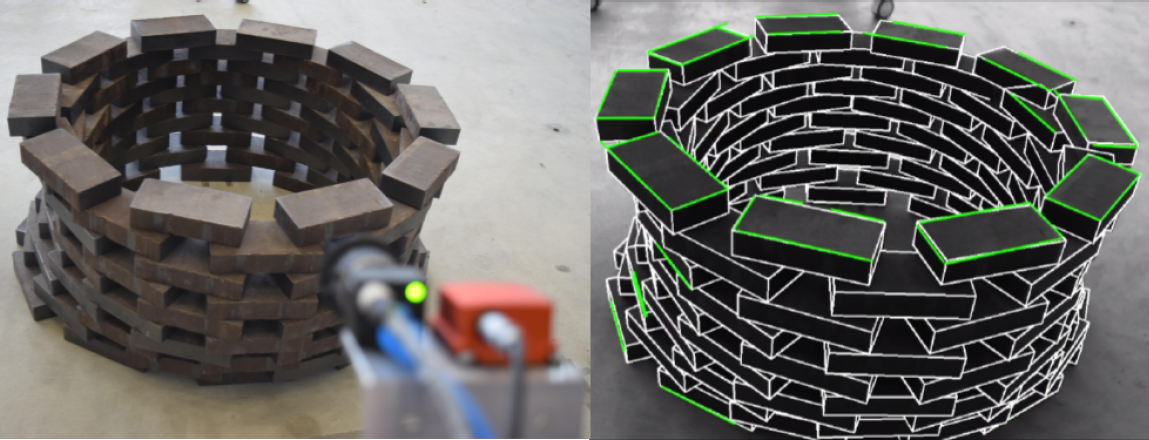
\includegraphics[width=0.9\linewidth]{figures/object_tracker_example.png}
    \caption[Object Tracker Brick Tower Showcase]{A brick tower built with the help of a visual-inertial tracking system. The left image shows the brick tower and the sensor-head while the right image shows the camera image overlaid with the rendered geometry. Directly taken from \cite{ViObjectTracker}.}
      \label{fig:objectTrackerExample}
\end{figure}

This work has since been further developed and currently consists of platform-independent \Cpp code and an application for Android phones. For the rest of this thesis we will refer to this code simply as the Object Tracker. The sensor fusion library used has since been open-sourced \cite{ConFusion} and the code further uses the ceres-solver~\cite{ceres-solver}, Eigen~\cite{eigen}, OpenCV~\cite{opencv_library} and Boost~\cite{boost} libraries.
\chapter{Results}

In thesis I create a port for the HoloLens 2 using the aforementioned Object Tracker. I use Research Mode \cite{ResearchMode} to provide the Object Tracker with the sensor data it needs and create a working application around it which runs on the HoloLens 2. In this chapter I will take a closer look at the indiviual components of my work.

\section{Sensor API}\label{sec:sensorapi}

At the heart of the application lies the Sensor API. It unifies several sensors from different APIs to provide raw data streams. The \lstinline{SensorApi} class serves as the interface between the Sensor API and the application that retrieves its data. It initializes the individual sensor interfaces with their respective APIs and manages them.

Each sensor is represented in the code by a sensor interface. Each sensor interface is running a separate thread in which it continuously loads new data. The \lstinline{SensorApi} class then provides functions for extracting this data by the application processing it. 

In the case of the IMU sensors, \lstinline{SensorApi} only exposes a single function which returns the merged IMU measurements instead of independent measurements for each individual sensor. The measurements from the IMU sensors usually don't arrive at the same time, let alone at the same frame rate. The \lstinline{SensorApi} therefore stores the measurements it receives in separate buffers and returns only complete IMU measurements (consisting of both accelerometer and gyroscope measurements) where data from both sensors has arrived. 

Furthermore the \lstinline{SensorApi} class exposes functions to retrieve extrinsic transformation matrices for all sensors. With these it is possible to create transformation matrices for transformations between any pair of sensors. As mentioned in sec. \ref{sec:ResearchMode}, all sensors are located relative to a rigid node which is determined by Research Mode. For example \lstinline{GetT_gyroscope_rigid()} would return a 4x4 transformation matrix which can be used to transform a vector from the coordinate system of the rigid node into the coordinate system of the gyroscope. For readers unfamiliar with this naming convention, I refer to the appendix sec. \ref{apx:naming}.

The whole Sensor API only uses Mixed Reality Windows APIs and Research mode. The conversion to Eigen, OpenCV and similar libraries used by the Object Tracker is done outside of the Sensor API. It is therefore possible to use this API as a plug and play module which can be integrated into projects with similar use cases.

A UML diagram of all the important classes, properties and methods can be found in fig. \ref{fig:SensorApiUML}. I have implemented interfaces for four different kinds of sensors which I describe briefly in the following subsections.

\begin{empfile}[SensorApiUML]
\begin{empcmds}
input metauml;
\end{empcmds}
\begin{empdef}[SensorApiUML](100,100)
    Class.SensorApi("SensorApi")
           ("-accelData: deque<ImuSensorDataStruct>",
            "-gyroData: deque<ImuSensorDataStruct>") 
            ("+InitializeSensors(): void",
             "+GetImuMeasurements(): deque<ImuMeasurement>",
             "+GetCameraFrame(): CameraFrame",
             "+GetDepthCameraFrame(): DepthCameraFrame",
             "+GetT_rigid_camera(): float4x4",
             "+GetT_accelerometer_rigid: float4x4",
             "+GetT_gyroscope_rigid: float4x4",
             "+GetT_depthCamera_rigid: float4x4");
             
    AbstractClass.ImuInterface("ImuInterface")
            ("#dataBuffer: deque<ImuSensorDataStruct>",
             "#sampleFrequency: int",
             "#updateThread: thread")
            ("+GetBuffer(): deque<ImuSensorDataStruct>",
             "+GetExtrinsics(): float4x4",
             "#GetDirectXExtrinsicsMatrx(): XMFLOAT4X4",
             "#GetSamples(): vector<ImuSensorDataStruct>");
    Class_stereotypes.ImuInterface("<<Research Mode>>");
             
    Class.AccelInterface("AccelInterface")
            ()
            ("#GetDirectXExtrinsicsMatrx(): XMFLOAT4X4",
             "#GetSamples(): vector<ImuSensorDataStruct>");
    Class_stereotypes.AccelInterface("<<Research Mode>>");
             
    Class.GyroInterface("GyroInterface")
            ()
            ("#GetDirectXExtrinsicsMatrx(): XMFLOAT4X4",
             "#GetSamples(): vector<ImuSensorDataStruct>");
    Class_stereotypes.GyroInterface("<<Research Mode>>");
             
    Class.CameraInterface("CameraInterface")
            ("-Trc: float4x4",
             "-lastFrame: CameraFrame")
            ("+GetLastFrame(): CameraFrame",
             "+GetExtrinsics(): float4x4");
             
    Class.DepthCameraInterface("DepthCameraInterface")
            ("-lastFrame: DepthCameraFrame",
             "-updateThread: thread")
            ("+GetLastFrame(): DepthCameraFrame",
             "+GetExtrinsics(): float4x4");
    Class_stereotypes.DepthCameraInterface("<<Research Mode>>");
    
    xPadding:=50;
    yPadding:=70;
    SensorApi.nw = (0,0);
    DepthCameraInterface.nw = atright(SensorApi.ne, xPadding);
    CameraInterface.nw = below(DepthCameraInterface.sw, 20);
    AccelInterface.nw = below(SensorApi.sw, yPadding);
    GyroInterface.nw = atright(AccelInterface.ne, xPadding);
    ImuInterface.nw = below(AccelInterface.sw, yPadding);
    
    drawObjects(SensorApi, ImuInterface, AccelInterface, GyroInterface, CameraInterface, DepthCameraInterface);
    link(aggregationUni)(DepthCameraInterface.w -- atleft(DepthCameraInterface.w, xPadding));
    link(aggregationUni)(CameraInterface.w -- atleft(CameraInterface.w, xPadding));
    link(aggregationUni)(AccelInterface.n -- above(AccelInterface.n, yPadding));
    link(aggregationUni)(GyroInterface.n -- atleft(SensorApi.se, 20));
    link(inheritance)(AccelInterface.s -- ImuInterface.n);
    link(inheritance)(GyroInterface.s -- ImuInterface.ne);
\end{empdef}
\end{empfile}
\begin{figure}
    \centering
    \empuse{SensorApiUML}
    \caption[UML Diagram of the Sensor API]{UML Diagram of the Sensor API: The \lstinline{SensorApi} class manages all sensor interfaces and exposes functions to retrieve data and extrinsic transformation matrices from them. The \lstinline{CameraInterface} class collects its data from Mixed Reality Windows APIs, all other sensor interfaces retrieve their data via Research Mode. \lstinline{ImuInterface} is an abstract class implementing all of the shared code for the sensor interfaces of the different IMU sensors. 
      \label{fig:SensorApiUML}}
\end{figure}

\subsection{Camera Interface}

The \lstinline{CameraInterface} class uses only Mixed Reality Windows APIs to retrive frames of the RGB camera of the HoloLens 2. It retrieves these frames at 30fps with a resolution of 960x540 but the resolution can be configured to be up to 1920x1080. It uses the GUID of the Research Mode rigid node provided by \lstinline{SensorApi} to locate the RGB camera relative to this rigid node. This transformation matrix has the form $T_{RC}$.

The returned \lstinline{CameraFrame} struct looks as follows:

\begin{lstlisting}
struct CameraFrame {
  uint64_t ts;
  SoftwareBitmap bitmap;
  float2 principalPoint;
  float2 focalLength;
  SpatialCoordinateSystem coordinateSystem;
};
\end{lstlisting}

The \lstinline{SoftwareBitmap} class defines all properties of the image, for example data, image width, image height and format. For convenience \lstinline{bitmap} is already converted to BGRA 8-Bit. \lstinline{coordinateSyste} is later used to calculate a transformation between the world coordinate system of the Object Tracker and the world coordinate system of the HoloLens.

\subsection{IMU Interfaces}

The \lstinline{AccelInterface} and \lstinline{GyroInterface} classes represent their respective Research Mode sensors. They share most of their code and therefore inherit it from an abstract super class \lstinline{ImuInterface}. The sensors themselves work at different frame rates and at each frame the Research Mode API returns a buffer of measurement samples. The interfaces then down sample the incoming measurements to a desired frequency, in my case 200 measurements per second. The measurements can than be retrieved as a vector of \lstinline{ImuSensorDataStruct} structs:

\begin{lstlisting}
struct ImuSensorDataStruct {
  uint64_t ts;
  float ImuValues[3];
};
\end{lstlisting}

These measurements are then merged by \lstinline{SensorApi} into \lstinline{ImuMeasurement} structs of the form:

\begin{lstlisting}
struct ImuMeasurement {
  uint64_t ts;
  float AccelValues[3];
  float GyroValues[3];
};
\end{lstlisting}

Extrinsic transformation matrices are retrieved directly from research mode and take the form $T_{AR}$ and $T_{GR}$ respectively.

While I didn't implement a sensor interface for the magnetometer since it is not needed for the Object Tracker, it should be trivial to do so since its Research Mode sensor shares most of its behaviour with the other IMU sensors.

\subsection{Depth Camera Interface}

As mentiond in sec. \ref{sec:holHardware}, \lstinline{DepthCameraInterface} has two possible modes of operation, AHAT or Long Throw. Which one to use is defined by \lstinline{SensorApi}. Independent of the mode, the interface can be queried  for the \lstinline{DepthCameraFrame} struct: 

\begin{lstlisting}
struct DepthCameraFrame {
  uint64_t ts;
  uint32_t width;
  uint32_t height;
  std::vector<uint16_t> depthData;
  std::vector<uint16_t> activeBrightnessImage;
};
\end{lstlisting}

Here \lstinline{depthData} is a vector of size \lstinline{width * height} containing the depth values for each pixel. Invalid pixels contain a value of 0. \lstinline{activeBrightnessImage} is a vector of the same size and contains the original infrared image used to calculate the depth map.

At the moment, this sensor is not used by the Object Tracker algorithm and therefore disabled in \lstinline{SensorApi}. However it is ready to be used at either a later point in time or by a different application.

\section{Object Tracker Integration}\label{sec:objectTrackerIntegration}

I now use the Sensor API to retrieve the raw sensor data and feed it into the Object Tracker. The main interface for the Object Tracker is the \lstinline{ObjectTracker} class which exposes various functions to interact with the library. To connect the \lstinline{ObjectTracker} and \lstinline{SensorApi} classes I have created the \lstinline{ViotApplication} class. This class first initiates an instance of \lstinline{SensorApi} and then waits for all sensors to be initialized and ready. Once that is the case, it initializes the \lstinline{ObjectTracker} by loading a configuration file. This file allows for the specification of various configurations such as brick size, which building plan to use and if a log file should be created.

Next the $T_{CameraIMU}$ transformation matrix needs to be set so the \lstinline{ObjectTracker} can transform IMU measurements to the camera space and vice-versa. Since the object tracker doesn't distinguish between different IMU sensors but treats them as a single sensor, we choose to define the IMU position as the position of the accelerometer. To calculate $T_{CameraIMU}$, we retrieve $T_{RigCamera}$ and $T_{AccelRig}$ from the Sensor API and set:

\begin{equation*}
    T_{CameraIMU} := T_{RigCamera}^{-1} * T_{AccelRig}^{-1}
\end{equation*}

The camera calibration also needs to be set in the \lstinline{ObjectTracker}. These parameters can be read directly from the current \lstinline{CameraFrame} provided by \lstinline{SensorApi}.

\lstinline{ViotApplication} runs a separate thread for the RGB camera, the depth camera and the IMU sensor each. Again, the depth camera thread is disabled because it is not needed at the current time. Whenever new data arrives, it is retrieved from the \lstinline{SensorApi} instance, transformed into the format \lstinline{ObjectTracker} expects, and fed into it. For example are IMU measurements converted to Eigen vectors and images are converted to OpenCV matrices. This process is shown in fig. \ref{fig:dataThreads}.

\begin{figure}
    \centering  
    \begin{sequencediagram}
        \newthread{ViotThread}{ViotApplication::SensorThread}
        \newinst{SensorApi}{SensorApi}
        \newinst{SensorInterface}{SensorInterface}
        \newthread{SensorThread}{SensorInterface::DataThread}
        
        \begin{call}{SensorThread}{WaitForData()}{SensorThread}{}
        \end{call}
        \begin{call}{SensorThread}{SaveData()}{SensorInterface}{}
        \end{call}
        \mess{SensorThread}{notify}{ViotThread}
        \begin{call}{ViotThread}{GetData()}{SensorApi}{return data}
            \begin{call}{SensorApi}{GetData()}{SensorInterface}{return data}
            \end{call}
        \end{call}
        \begin{call}{ViotThread}{AddToObjectTracker(data)}{ViotThread}{}
        \end{call}
        \begin{call}{SensorThread}{WaitForData()}{SensorThread}{}
        \end{call}
    \end{sequencediagram}
    \caption[Abstracted sequence diagram of data thread interactions]{Abstracted sequence diagram of data thread interactions: Each sensor interface runs a thread to continuously fetch data from its sensor which is then saved in the sensor interface instance. After that, the respective thread of the \lstinline{ViotApplication} instance is notified which then retrieves the data from the sensor interface via the \lstinline{SensorApi} and feeds it into the \lstinline{ObjectTracker}. \lstinline{ViotApplication} runs one thread for each sensor type.}
    \label{fig:dataThreads}
\end{figure}

Since the position of the accelerometer is treated as the IMU position, gyroscope measurements need to be transformed into the accelerometer space. For this the rotation matrices $R_{AccelRig}$ and $R_{GyroRig}$ are extracted from $T_{AccelRig}$ and $T_{GyroRig}$ respectively which are retrieved from the \lstinline{SensorApi}. All gyroscope measurements are then rotated by:

\begin{equation*}
    R_{AccelGyro} = R_{AccelRig} * R_{GyroRig}^{-1}
\end{equation*}

It is not necessary to perform use the full transformation matrix (i.e. include the translation) because gyroscope measurements are translation invariant.

Because IMU measurements can lag behind camera frames by up to 0.3 seconds, camera frames are stored in a buffer and only fed into the \lstinline{ObjectTracker} when the corresponding IMU measurements have arrived. This way \lstinline{ObjectTracker} doesn't wait idly for IMU measurements to arrive but optimizes the last available state. 

After feeding camera frames into the \lstinline{ObjectTracker}, \lstinline{ViotApplication} retrieves the latest estimation for $T_{WorldIMU}$ by the \lstinline{ObjectTracker}. The pose of the camera at the same time is then used to calculate the estimated transformation matrix from the HoloLens world to the Object Tracker world. This is necessary to be able to transform objects from the world coordinate system of the Object Tracker in which they are tracked into the world coordinate system of the HoloLens in which they are drawn.

The user interface thread of the application calls the \lstinline{Update()} and \lstinline{Draw()} functions of \lstinline{ViotApplication} once every iteration. During \lstinline{Update()} the poses of all objects are updated with the estimates provided by the \lstinline{ObjectTracker} while \lstinline{Draw()} draws them into the holographic space.

An UML diagram of the this part of the application can be seen in fig. \ref{fig:ObjectTrackerUML}.

\begin{empfile}[ObjectTrackerUML]
\begin{empcmds}
input metauml;
\end{empcmds}
\begin{empdef}[ObjectTrackerUML](100,100)
    Class.SensorApi("SensorApi")
           () 
            ("+GetImuMeasurements(): deque<ImuMeasurement>",
             "+GetCameraFrame(): CameraFrame",
             "+GetDepthCameraFrame(): DepthCameraFrame",
             "+GetT_rigid_camera(): float4x4",
             "+GetT_accelerometer_rigid: float4x4",
             "+GetT_gyroscope_rigid: float4x4",
             "+GetT_depthCamera_rigid: float4x4");
             
    Class.ViotApplication("ViotApplication")
            ("-imuThread: thread",
             "-cameraThread: thread",
             "-depthThread: thread",
             "-cameraBuffer: deque",
             "-drawDebugImage: bool")
            ("+StartPoseInitialization(): void",
             "+EndPoseInitialization(): void",
             "+RequestStep(): void",
             "+RequestStepBack(): void",
             "+StopTracking(): void",
             "+ToggleFullPlan(): void",
             "+GetTrackerState(): TrackerState",
             "+Update(): void",
             "+Draw(): void");
            
    Class.ObjectTracker("ObjectTracker")
            ()
            ("+addImuMeasurement(ts:double, accel:Vector3, gyro:Vector3): void",
             "+addImage(ts:double, image:Mat): void",
             "+setTciExternally(Tci:Pose): void()",
             "+setCameraCalibration(focal:float2, principal:float2, height:int, width:int): void",
             "+state(): TrackerState",
             "+startPoseInit(): void",
             "+donePoseInit(): void",
             "+stepRequest(): void",
             "+stepBackRequest(): void",
             "+stopTrackingRequest(): void",
             "+setVisualizFullBuildingPlan(show:bool): void",
             "+GetPendingObjectPose(): Pose",
             "+GetMostRecentObjectPoses(): vector<Pose>",
             "+getLatestTwiEstimate(Twi:Pose, ts:double): void");
    
    topToBottom(70)(SensorApi, ViotApplication, ObjectTracker);
    
    drawObjects(ViotApplication, SensorApi, ObjectTracker);
    
    link(aggregationUni)(SensorApi.s -- ViotApplication.n);
    link(aggregationUni)(ObjectTracker.n -- ViotApplication.s);
\end{empdef}
\end{empfile}
\begin{figure}
    \centering
    \empuse{ObjectTrackerUML}
    \caption[UML Diagram of the Object Tracker integration]{UML Diagram of the Object Tracker integration: The \lstinline{ViotApplication} class retrieves data from the \lstinline{SensorApi}, transforms it into the correct format and feeds it into the \lstinline{ObjectTracker}. It is also responsible for updating and drawing tracked objects retrieved from \lstinline{ObjectTracker}.
      \label{fig:ObjectTrackerUML}}
\end{figure}

\subsection{User Interface}

The user interface consists of five buttons which are either enabled or disabled depending on the current state of the Object Tracker. The Object Tracker can be in one of three states:

\begin{itemize}
    \item HOLD: The Object Tracker is idle and waits for tracking to start.
    \item INIT: The Object Tracker is in the process of being initialized. In this state the user can place the first brick and start tracking when he or she is finished.
    \item TRACKING: The Object Tracker is in the process of tracking. 
\end{itemize}

The five buttons are:

\begin{itemize}
    \item Start Init: This button starts the pose initialization of the Object Tracker. This means, the first brick will be drawn and move with the users head.
    \item Done Init: Once the brick moving with the users head is correctly positioned, this button may be pressed to lock it in place. This starts the tracking of the brick.
    \item Next: This button goes one step forward. This means that if all active objects have been placed, a new pending object is added and if a pending object is ready to be tracked, it changes this object's state from pending to active. 
    \item Back: This button does the reverse of the Next button.
    \item Stop: This button stops the tracking.
\end{itemize}

The state of each button depending on the state of the Object Tracker can be found in tab. \ref{tab:buttonStates}.

\begin{table}
\centering
\begin{tabular}{ | l | c | c | c | c | c | }
 \hline
 & \textbf{Start Init} & \textbf{Done Init} & \textbf{Next} & \textbf{Back} & \textbf{Stop} \\
 \hline
 \textbf{HOLD} & \checkmark & \text{\sffamily X} & \text{\sffamily X} & \text{\sffamily X} & \text{\sffamily X} \\
 \textbf{INIT} & \text{\sffamily X} & \checkmark & \text{\sffamily X} & \text{\sffamily X} & \checkmark \\
 \textbf{TRACKING} & \text{\sffamily X} & \text{\sffamily X} & \checkmark & \checkmark & \checkmark \\
 \hline
\end{tabular}
\caption[Active UI buttons depending on the Object Tracker state]{The state of each button of the user interface depending on the current state of the Object Tracker. A checkmark means that the button is enabled in this state, while an \text{\sffamily X} means it is disabled.}
\label{tab:buttonStates}
\end{table}

The buttons are placed in a row on the lower part of the users viewport. A screenshot can be seen in fig. \ref{fig:ui}. The state transitions in the object tracker triggered by the buttons can be seen in fig. \ref{fig:ObjectTrackerStates}.

\begin{figure}
    \centering
    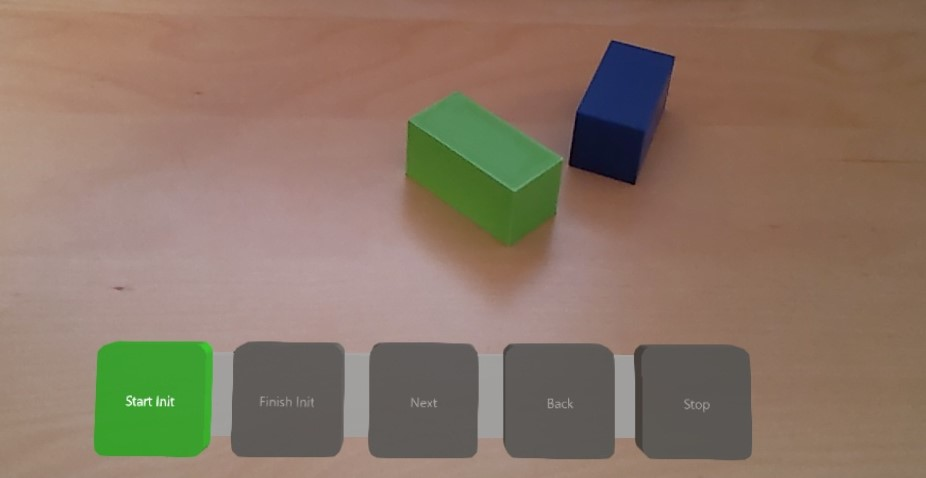
\includegraphics[width=0.9\linewidth]{figures/hololens_ui.jpg}
    \caption[Screenshot of the user interface]{Screenshot of the user interface: The buttons are lined up on the bottom half of the viewport and enabled or disabled depending on the state of the object tracker. In this case, only the first button is enabled.}
      \label{fig:ui}
\end{figure}

\begin{empfile}[ObjectTrackerStates]
\begin{empcmds}
input metauml;
\end{empcmds}
\begin{empdef}[ObjectTrackerStates](100,100)
    State.Hold("HOLD")();
    State.Init("INIT")();
    State.Tracking("TRACKING")();
    
    boxit.Start("StartInit");
    boxit.Done("DoneInit");
    boxit.Next("Next");
    boxit.Back("Back");
    boxit.Stop1("Stop");
    boxit.Stop2("Stop");
    
    leftToRight(70)(Hold, Init, Tracking);
    
    Start.s = above(atright(Hold.e, 35), 5);
    Done.s = above(atright(Init.e, 35), 5);
    Stop1.s = above(Init.n, 25);
    Stop2.n = below(atright(Hold.se, 35), 25);
    Next.n = below(Tracking.s, 30);
    Back.n = below(Tracking.s, 40);
    
    drawObjects(Hold, Init, Tracking);
    drawunboxed(Start, Done, Next, Back, Stop1, Stop2);
    link(transition)(Hold.e -- Init.w);
    link(transition)(Init.e -- Tracking.w);
    link(transition)(pathCut(Tracking, Hold)(Tracking.n -- above(Tracking.n, 20) -- above(Hold.n, 20) -- Hold.n));
    link(transition)(pathCut(Init, Hold)(Init.s -- below(Init.s, 20) -- below(Hold.s, 20) -- Hold.s));
    link(transition)(atleft(Tracking.s, 5) .. below(Tracking.s, 30) .. atright(Tracking.s, 5));
\end{empdef}
\end{empfile}
\begin{figure}
    \centering
    \empuse{ObjectTrackerStates}
    \caption[State transition diagram for the object tracker UI]{State transition diagram for the object tracker UI: Boxes represent the possible states the object tracker can be in while transitions represent button presses in the user interface.
      \label{fig:ObjectTrackerStates}}
\end{figure}

When a brick is not positioned correctly the Object Tracker provides poses for arrows which are then drawn at the corners of the brick. This helps the user to correct the position.

\subsection{Debug Screen}

\begin{figure}
    \centering
    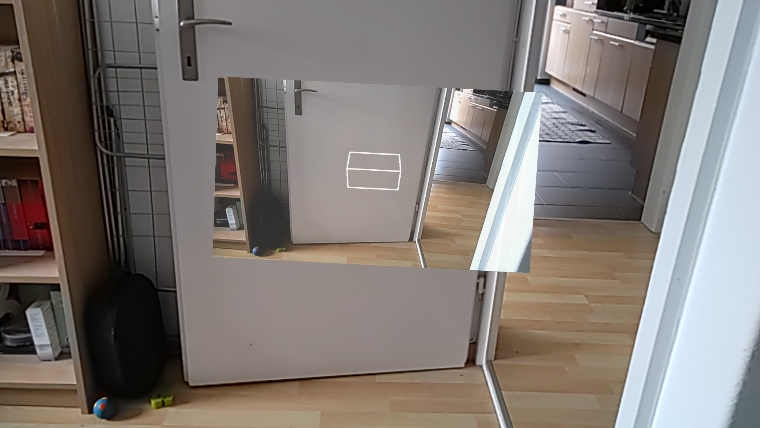
\includegraphics[width=0.9\linewidth]{figures/debug_screen.jpg}
    \caption[Debug Screen for Development]{This image shows the debug screen which can be enabled in \lstinline{ViotApplication} debugging and easier development}
      \label{fig:debugScreen}
\end{figure}

To help with development and debugging, I also provide a debug screen which can be enabled in \lstinline{ViotApplication}. It draws a virtual screen which moves with the user's head and can display any image required. It is especially useful for showing what the Object Tracker would render but it can be configured to show any other image stream.

\subsection{Showcase}

\begin{figure}
    \centering
    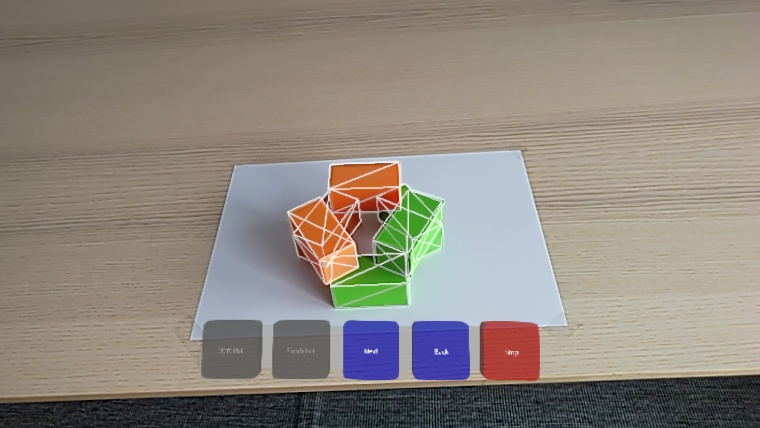
\includegraphics[width=0.9\linewidth]{figures/teaser.jpg}
    \caption[Showcase]{Brick tower built with the Object Tracker on the HoloLens 2. The image shows a screenshot of the HoloLens 2.}
      \label{fig:showcase}
\end{figure}

Fig. \ref{fig:showcase} shows a brick tower built with application presented in this thesis. A video of the complete build process is linked in appendix sec. \ref{apx:video}.

\section{Limitations}

As already mentioned in sec. \ref{sec:objectTrackerIntegration} the IMU measurements provided by Research Mode generally lag up to 0.3 seconds behind the camera frame. Because of this, camera frames have to be held back until the corresponding IMU measurements have arrived. This, of course leads to noticeable delays in the information retrieved from the Object Tracker. Furthermore, while it is possible to use large numbers of IMU measurements per second (I use 200 for this application but larger numbers are possible), these measurements arrive in large batches but at a low frame rate of between 12Hz to 22Hz which leads to the input of a lot of measurements simultaneously. It would be preferred to provide these measurements in a more continuous stream.

The most noticeable limitation imposed by the delayed IMU measurements occurs during the initialisation of the first object pose. It is decidedly more challenging because the pose which should move with the head of the user has a noticeable delay. Once the first pose is initialized it gets better but from time to time one can still notice delayed readjustments of the brick poses to head movement. 

Another limitation is the computing power of the HoloLens 2 in general. Because of this, the Object Tracker often needs longer to optimize than it would on a modern phone. This can lead to even more delayed adjustments, general instability or even loss of tracking.
\chapter{Conclusion and Outlook}

In this thesis I presented an integration of the Object Tracker for the HoloLens 2 ecosystem. I presented the Sensor API, an interface to get data streams from various HoloLens 2 sensors via sensor interfaces which use standard Windows APIs and Research Mode. Because I don't use any other libraries than standard Windows APIs and Research Mode in the Sensor API, it can easily be used for different projects with the similar requirements.

I then used these raw data streams to incorporate the Object Tracker into a mixed reality application which provides a simple user interface to interact with the Object Tracker. I also used the Cannon library to display bricks tracked by the Object Tracker in the holographic space which allows for the user to accurately build a simple brick tower by hand.

The current application can be improved further in a couple of different ways. For one, the Object Tracker could make use of the depth camera of the HoloLens 2. The Sensor API already provides an interface to retrieve this data however it is not yet used by the Object Tracker.

Another point of improvement is Research Mode itself. While it grants access to low-level sensor streams which are otherwise not available, the API is not yet optimized for applications working in real-time. For one, IMU measurements retrieved via Research Mode always lag a couple of tenths of a second behind real-time. This introduces lag into the application which makes it more difficult to perform real-time taks. While it is possible to retrieve a lot of measurement samples per second for every IMU sensor, these measurement samples arrive in batches at low frame rates which reduces some of the advantages of having many samples per second available. If Microsoft decides to improve Research Mode in the future, such changes would have a large impact on real-time object tracking.

Finally, the performance of the Object Tracker on the HoloLens 2 is not as good as on other platforms because of limited computational power. Some of the optimization steps take a lot of time which can result in delayed adjustments and general instability. This could be improved by looking at ways to optimize the Object Tracker further, especially in regard of the ecosytem of the HoloLens 2. It is also to be expected that future generations of mixed reality headsets will have more computational power which will of course diminish this effect.


% ---- END MAIN PART ----


\appendix
\clearpage
\renewcommand*{\chapterpagestyle}{myappendixpagestyle}

\chapter{Appendix}

\section{Showcase Video}\label{apx:video}

I recorded a short video showcasing my work. I uploaded the video to YouTube and it can be found at \url{https://youtu.be/wArK9bmHatM}.

\section{Source Code}

The code written for this thesis is included within the Object Tracker code repository. It includes a section within the Readme with instructions on how to set it up and how to build and run it.

Since the code of the Object Tracker is proprietary, its Github repository is private and the code will not be released to the public. However the Sensor API part of the code (see sec. \ref{sec:sensorapi}) is designed to be compatible with any HoloLens 2 application using Research Mode and can be provided to interested parties.

\section{Transformation Matrix Naming Convention}\label{apx:naming}

The transformation matrices in this thesis follow the simple convention that $T_{AB}$ is a transformation matrix which transforms a vector from the coordinate system $B$ into the coordinate system $A$, i.e.:

\begin{equation*}
    x_A = T_{AB} * x_B
\end{equation*}

where $x_B$ is a vector in coordinate system $B$ and $x_A$ is the corresponding vector in coordinate system $A$.

Similarly $R_{AB}$ denotes a rotation matrix from coordinate system $B$ into the coordinate system $A$.

\clearpage
\renewcommand*{\chapterpagestyle}{empty}

%\nocite{*}
\cleardoublepage
\phantomsection
\addcontentsline{toc}{chapter}{Bibliography}
\bibliography{bibliography}

\cleardoublepage
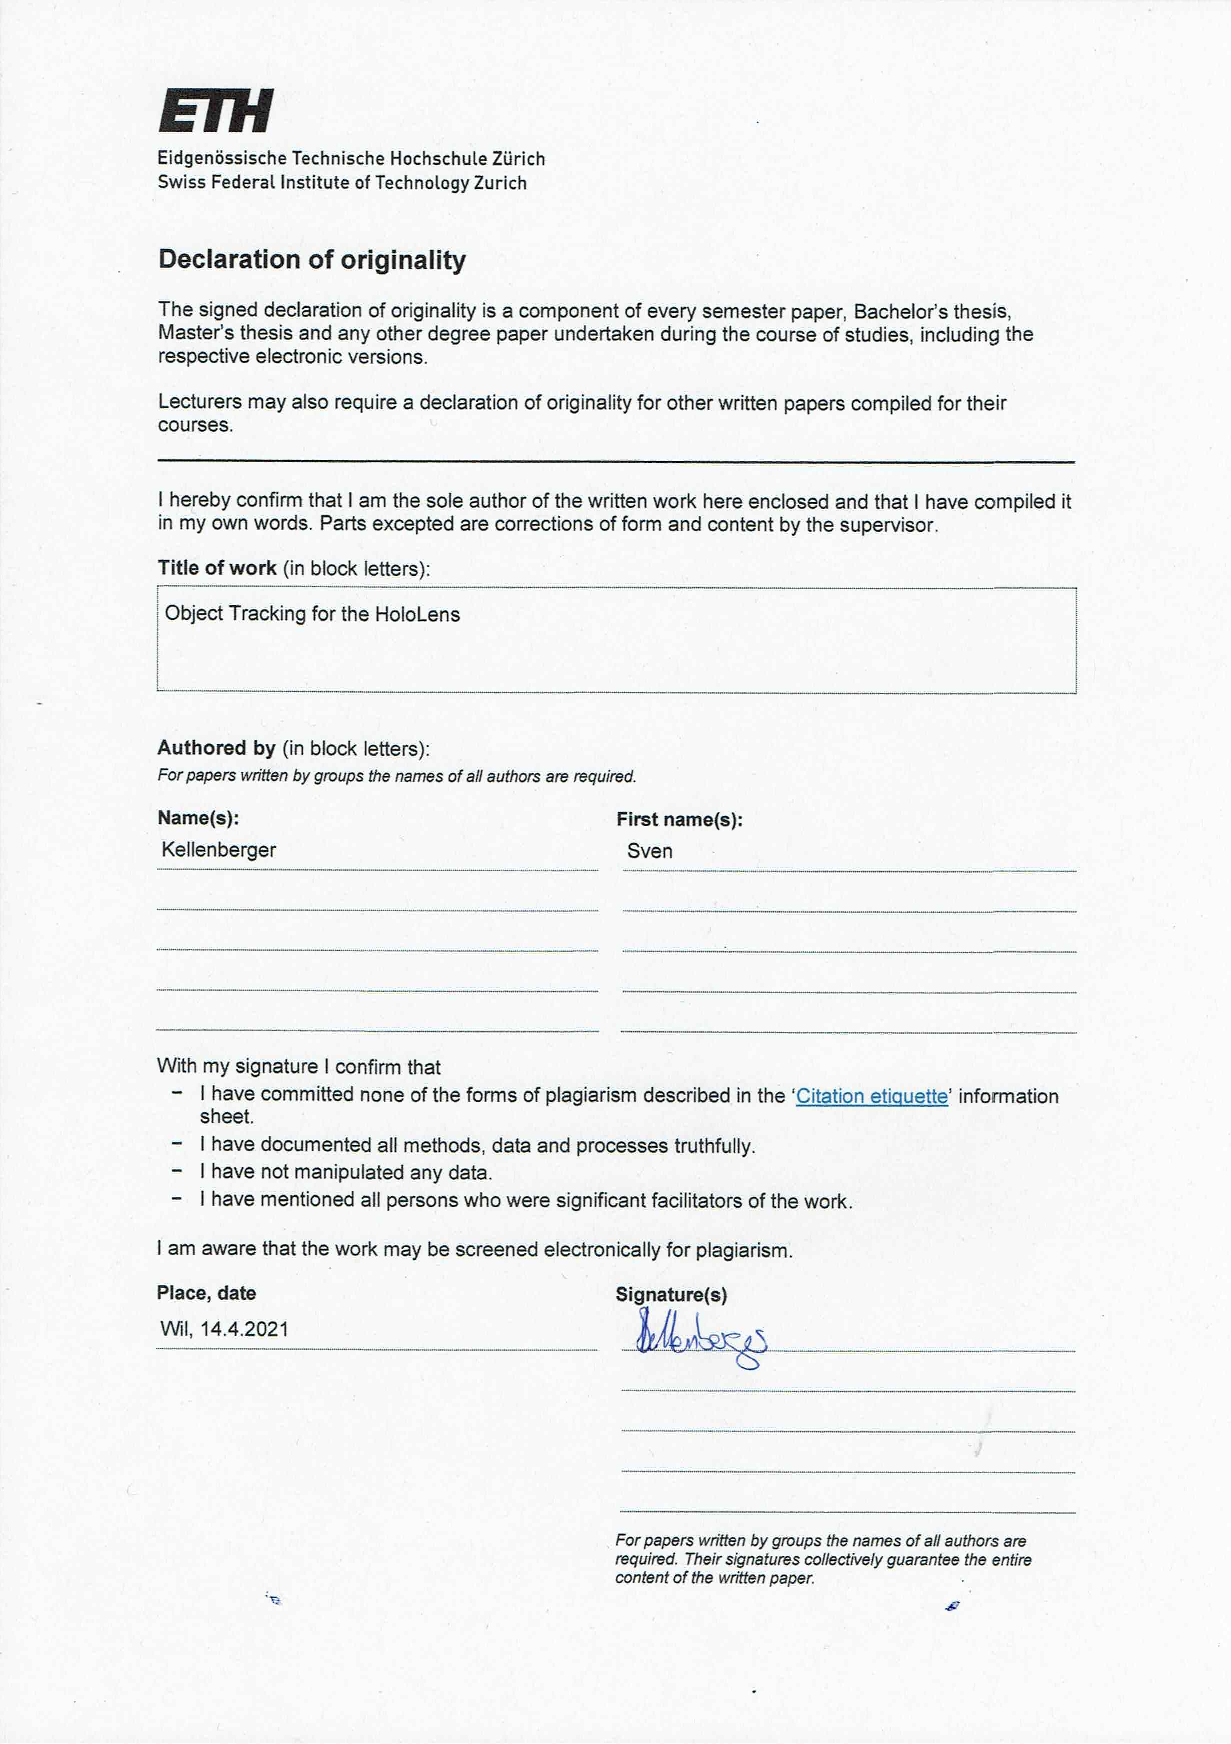
\includepdf{declaration-originality.pdf}

\end{document}
